
\documentclass[11pt,a4paper]{article}
\usepackage[margin=0.72in]{geometry}
\usepackage[T1]{fontenc}
\usepackage{lmodern}
\usepackage{xcolor}
\usepackage{hyperref}
\usepackage{enumitem}
\usepackage{booktabs,tabularx,array}
\usepackage{tikz}
\usetikzlibrary{arrows.meta,positioning,shapes.geometric,fit,calc}
\usepackage{fancyhdr}
\usepackage{titlesec}
\hypersetup{colorlinks=true,linkcolor=teal,urlcolor=blue}
\definecolor{teal}{RGB}{0,105,105}
\definecolor{pale}{RGB}{230,245,243}
\definecolor{dark}{RGB}{35,48,56}
\pagestyle{fancy}\fancyhf{}\lhead{Ovvasjatra — Project Proposal}\rhead{Software Engineering}\cfoot{\thepage}
\setlength{\headheight}{14pt}
\titleformat{\section}{\large\bfseries\color{teal}}{\thesection}{0.6em}{}
\titleformat{\subsection}{\normalsize\bfseries\color{dark}}{\thesubsection}{0.6em}{}
\setlist{nosep,leftmargin=1.5em}
\tikzset{
 box/.style={draw=teal,rounded corners=2pt,fill=pale,align=center,minimum height=7mm,text width=28mm,font=\small},
 entity/.style={draw=dark,fill=white,align=center,minimum width=25mm,minimum height=8mm,font=\small},
 process/.style={draw=teal,rounded corners=8pt,fill=pale,align=center,text width=30mm,minimum height=9mm,font=\small},
 arrow/.style={-{Stealth[length=2mm]},thick,draw=dark},
 uml/.style={draw=dark,fill=white,align=left,font=\scriptsize,text width=38mm,inner sep=3pt},
 actor/.style={draw=dark,ellipse,fill=white,align=center,minimum width=18mm,minimum height=8mm,font=\small}
}
\begin{document}
\begin{titlepage}
\centering
\vspace*{1.1cm}
{\Large\bfseries SOFTWARE PROJECT PROPOSAL\par}
\vspace{1.0cm}
{\Huge\bfseries\color{teal} Ovvasjatra\par}
\vspace{0.25cm}
{\Large A Simple Habit Tracker Application in Java\par}
\vspace{0.8cm}
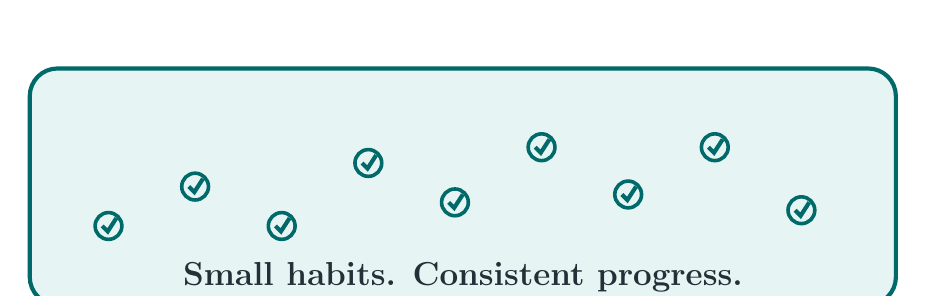
\begin{tikzpicture}
\draw[teal,line width=1.5pt,rounded corners=10pt,fill=pale] (0,0) rectangle (11,3.0);
\foreach \x/\y in {1/1,2.1/1.5,3.2/1,4.3/1.8,5.4/1.3,6.5/2,7.6/1.4,8.7/2,9.8/1.2} {
  \draw[teal,line width=1.3pt] (\x,\y) circle (0.17);
  \draw[teal,line width=1.5pt] (\x-0.08,\y) -- (\x-0.01,\y-0.07) -- (\x+0.1,\y+0.1);
}
\node[font=\large\bfseries,color=dark] at (5.5,0.35) {Small habits. Consistent progress.};
\end{tikzpicture}
\vspace{1.0cm}

\begin{tabular}{>{\bfseries}rl}
Project title: & Ovvasjatra (Habit Journey)\\
Language / UI: & Java, Java Swing\\
Process model: & Iterative and Incremental Model\\
Estimated duration: & 8 weeks\\
Student: & Ishtiak Ahmed Ayon\\
Student ID : & IT24039 \\
Department / University: & ICT / MBSTU\\
Course : & Software Engineering and Project Management\\
GitHub repository: & \url{https://github.com/ishtiakahmedayon/SEPM-Capstone-Project}
\end{tabular}

\vfill
{\small Initial proposal version 1.0 \quad|\quad 26 October 2026}
\end{titlepage}

\tableofcontents
\newpage

\section{Executive Summary}
Ovvasjatra (অভ্যাসযাত্রা, meaning ``habit journey'') is a lightweight Java desktop application that helps a user build consistent routines. A user can create habits, set a frequency or daily target, record completion for a date, and review a simple progress summary. The initial version focuses on a clear interface and reliable local storage rather than social features or cloud accounts.

\section{Problem Statement and Motivation}
People often begin routines but struggle to track consistency over time. Paper notes and generic to-do lists do not always provide a dedicated view of recurring habits. Ovvasjatra will provide a small, focused tool to record habits and see completion progress. The project is suitable for an individual software engineering project because it includes requirements analysis, design diagrams, object-oriented implementation, testing, and documentation.

\section{Objectives and Scope}
\subsection{Objectives}
\begin{itemize}
\item Create, view, edit, and archive personal habits.
\item Record whether a habit is completed on a selected day.
\item Show a daily checklist and basic completion statistics.
\item Store data locally so it remains available after restarting the app.
\item Apply object-oriented design and test the core use cases.
\end{itemize}
\subsection{In Scope}
Single-user desktop use; habit name and description; daily/weekly frequency; completion records; simple streak/percentage summary; local persistence; input validation.
\subsection{Out of Scope for Version 1}
Cloud synchronisation, multiple accounts, social sharing, mobile apps, push notifications, AI recommendations, and integrations with wearable devices.

\section{Stakeholders and Users}
\begin{tabularx}{\linewidth}{lX}
\toprule
Stakeholder & Interest / responsibility\\ \midrule
Primary user & Creates habits, logs completion, reviews progress.\\
Student developer & Analyses requirements, designs, implements, tests, and documents the app.\\
Course instructor / supervisor & Reviews proposal, milestones, diagrams, and final demonstration.\\
\bottomrule
\end{tabularx}

\section{Requirements}
\subsection{Functional Requirements}
\begin{tabularx}{\linewidth}{p{1.5cm}X}
\toprule
ID & Requirement\\ \midrule
FR-01 & The user can add a habit with a name, description, and frequency.\\
FR-02 & The user can view all active habits in a list.\\
FR-03 & The user can edit or archive a habit.\\
FR-04 & The user can mark a habit complete or undo completion for a date.\\
FR-05 & The app displays completed/total habits and a completion percentage for the selected day.\\
FR-06 & Habit details and completion records persist locally between launches.\\
FR-07 & The app validates required fields and gives understandable error messages.\\
\bottomrule
\end{tabularx}
\subsection{Non-functional Requirements}
\begin{itemize}
\item Usability: common actions should be understandable without training.
\item Reliability: completion records should not be lost during normal application exit.
\item Performance: display a typical personal habit list in under one second on a standard student PC.
\item Maintainability: separate UI, business logic, and persistence responsibilities.
\item Privacy: version 1 stores data locally and does not transmit personal data.
\item Compatibility: Java 17 or later with a desktop environment supporting Swing.
\end{itemize}

\section{Software Process Model}
The project will use the \textbf{Iterative and Incremental Model}. Each iteration delivers a small working increment, receives feedback, and refines the next increment. This is appropriate for a small student project because the interface and requirements can be improved after early demonstrations.

\begin{center}
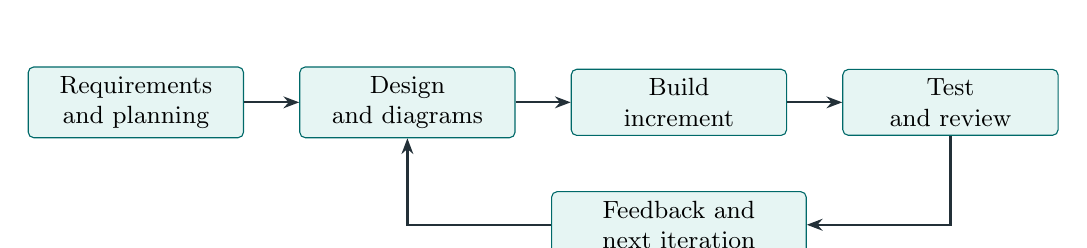
\begin{tikzpicture}[node distance=7mm and 7mm]
\node[box,text width=25mm] (req) {Requirements\\and planning};
\node[box,right=of req,text width=25mm] (design) {Design\\and diagrams};
\node[box,right=of design,text width=25mm] (build) {Build\\increment};
\node[box,right=of build,text width=25mm] (test) {Test\\and review};
\node[box,below=of build,text width=30mm] (feedback) {Feedback and\\next iteration};
\draw[arrow] (req)--(design);\draw[arrow] (design)--(build);\draw[arrow] (build)--(test);
\draw[arrow] (test)|-(feedback);\draw[arrow] (feedback)-|(design);
\end{tikzpicture}
\end{center}

\section{Project Schedule, Milestones, and Deliverables}
The schedule is an estimate for an eight-week individual project. Weeks may be adjusted with supervisor feedback.
\begin{tabularx}{\linewidth}{p{1.1cm}p{2.4cm}X p{2.3cm}}
\toprule
Week & Activity & Main output & Milestone\\ \midrule
1 & Idea and requirements & Proposal draft, requirements list & M1: Scope approved\\
2 & Analysis and design & DFD, use case, activity, ERD, UML drafts & M2: Design reviewed\\
3 & UI prototype & Swing screens and navigation & M3: UI demo\\
4 & Habit management & Add, list, edit, archive habits & M4: Habit CRUD\\
5 & Completion tracking & Daily completion and summary logic & M5: Tracking works\\
6 & Persistence & Local storage and validation & M6: Data persists\\
7 & Testing and refinement & Test cases, bug fixes, usability pass & M7: Test pass\\
8 & Final documentation & Final PDF, source code, README, demo & M8: Submission\\
\bottomrule
\end{tabularx}

\subsection{Gantt Chart}
\begin{center}
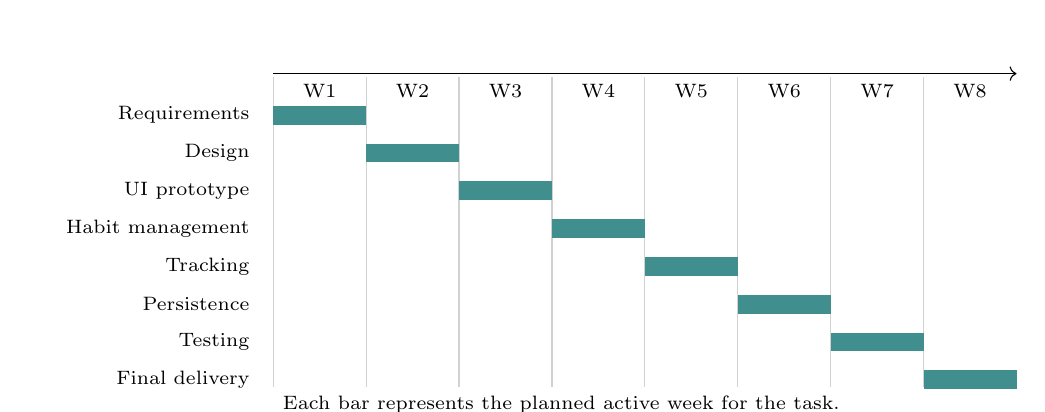
\begin{tikzpicture}[x=1.18cm,y=0.48cm,font=\scriptsize]
\foreach \w in {1,...,8} {
 \draw[gray!35] (\w,0) -- (\w,-8.2);
 \node at (\w+0.5,-0.35) {W\w};
}
\foreach \i/\lab in {1/Requirements,2/Design,3/UI prototype,4/Habit management,5/Tracking,6/Persistence,7/Testing,8/Final delivery} {
 \node[anchor=east,text width=2.7cm,align=right] at (0.85,-\i) {\lab};
}
\foreach \x/\y/\len in {1/1/1,2/2/1,3/3/1,4/4/1,5/5/1,6/6/1,7/7/1,8/8/1} {
 \fill[teal!75] (\x,-\y-0.25) rectangle (\x+\len,-\y+0.25);
}
\draw[->] (1,0.1)--(9,0.1);
\node[anchor=west] at (1,-8.65) {Each bar represents the planned active week for the task.};
\end{tikzpicture}
\end{center}

\section{System Design Diagrams}
\subsection{Data Flow Diagram (Level 0)}
\begin{center}
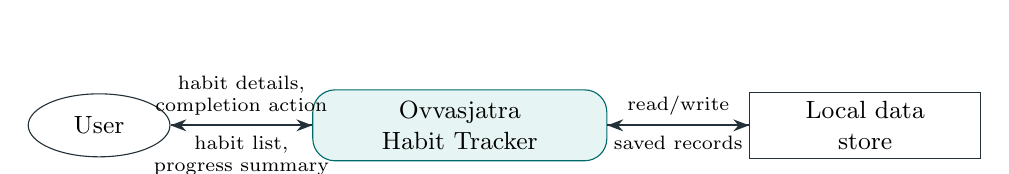
\begin{tikzpicture}[node distance=18mm]
\node[actor] (user) {User};
\node[process,right=of user,text width=35mm] (app) {Ovvasjatra\\Habit Tracker};
\node[entity,right=of app,text width=27mm] (store) {Local data\\store};
\draw[arrow] (user)--node[above,font=\scriptsize,align=center]{habit details,\\completion action}(app);
\draw[arrow] (app)--node[below,font=\scriptsize,align=center]{habit list,\\progress summary}(user);
\draw[arrow] (app)--node[above,font=\scriptsize]{read/write}(store);
\draw[arrow] (store)--node[below,font=\scriptsize]{saved records}(app);
\end{tikzpicture}
\end{center}

\subsection{Use Case Diagram}
\begin{center}
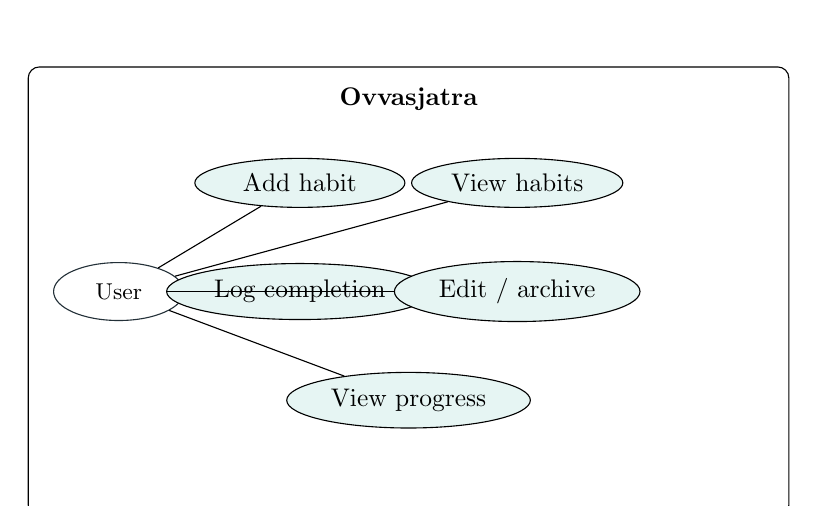
\begin{tikzpicture}[scale=.92,transform shape]
\node[draw,rounded corners,minimum width=105mm,minimum height=62mm] (sys) at (3.0,0) {};
\node[font=\bfseries] at (3,2.65) {Ovvasjatra};
\node[actor] (actor) at (-1,0) {User};
\node[ellipse,draw,fill=pale,minimum width=29mm] (add) at (1.5,1.5) {Add habit};
\node[ellipse,draw,fill=pale,minimum width=29mm] (view) at (4.5,1.5) {View habits};
\node[ellipse,draw,fill=pale,minimum width=29mm] (mark) at (1.5,0) {Log completion};
\node[ellipse,draw,fill=pale,minimum width=29mm] (edit) at (4.5,0) {Edit / archive};
\node[ellipse,draw,fill=pale,minimum width=29mm] (stats) at (3,-1.5) {View progress};
\draw (actor)--(add);\draw (actor)--(view);\draw (actor)--(mark);\draw (actor)--(edit);\draw (actor)--(stats);
\end{tikzpicture}
\end{center}

\subsection{Activity Diagram: Logging a Habit}
\begin{center}
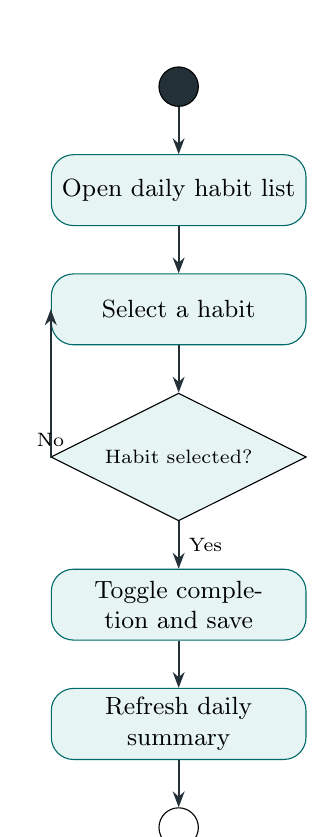
\begin{tikzpicture}[node distance=6mm]
\node[draw,circle,fill=dark,minimum size=5mm] (start) {};
\node[process,below=of start] (open) {Open daily habit list};
\node[process,below=of open] (select) {Select a habit};
\node[diamond,draw,fill=pale,aspect=2,below=of select,text width=22mm,align=center,font=\scriptsize] (valid) {Habit selected?};
\node[process,below=of valid] (save) {Toggle completion and save};
\node[process,below=of save] (update) {Refresh daily summary};
\node[draw,circle,fill=white,minimum size=5mm,below=of update] (end) {};
\draw[arrow] (start)--(open);\draw[arrow] (open)--(select);\draw[arrow] (select)--(valid);
\draw[arrow] (valid)--node[right,font=\scriptsize]{Yes}(save);
\draw[arrow] (save)--(update);\draw[arrow] (update)--(end);
\draw[arrow] (valid.west)-|node[near start,above,font=\scriptsize]{No}(select.west);
\end{tikzpicture}
\end{center}

\subsection{Entity Relationship Diagram (ERD)}
\begin{center}
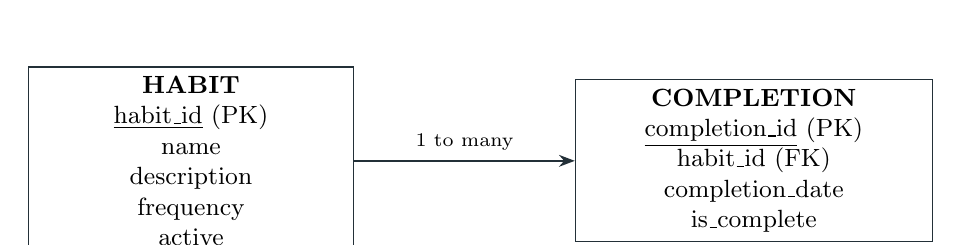
\begin{tikzpicture}[node distance=28mm]
\node[entity,text width=39mm] (habit) {\textbf{HABIT}\\\underline{habit\_id} (PK)\\name\\description\\frequency\\active};
\node[entity,right=of habit,text width=43mm] (log) {\textbf{COMPLETION}\\\underline{completion\_id} (PK)\\habit\_id (FK)\\completion\_date\\is\_complete};
\draw[arrow] (habit)--node[above,font=\scriptsize]{1 to many}(log);
\end{tikzpicture}
\end{center}
One habit can have many dated completion records. The combination of habit and date should be unique to prevent duplicate logs.

\subsection{Class Diagram}
\begin{center}
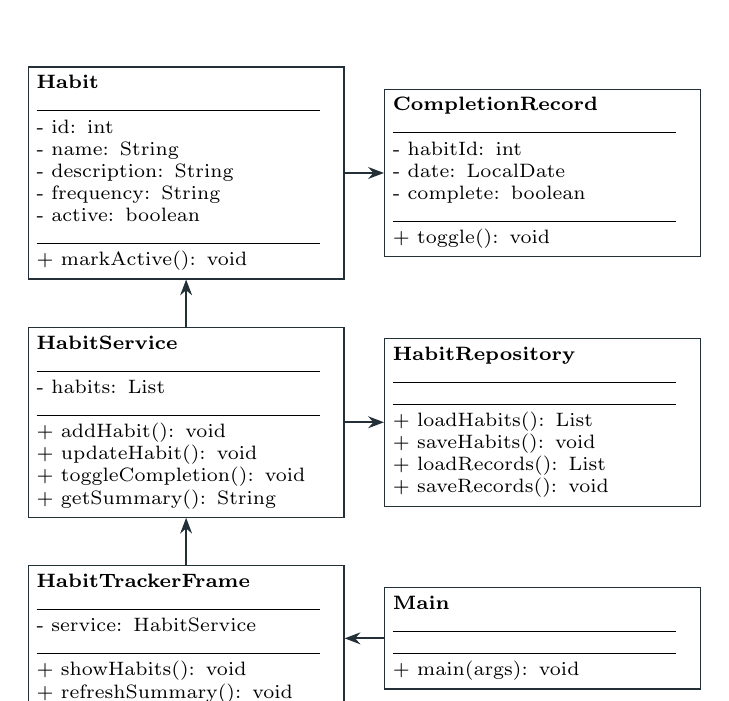
\begin{tikzpicture}[node distance=6mm and 5mm]
\node[uml] (habit) {\textbf{Habit}\\\rule{36mm}{.2pt}\\- id: int\\- name: String\\- description: String\\- frequency: String\\- active: boolean\\\rule{36mm}{.2pt}\\+ markActive(): void};
\node[uml,right=of habit] (log) {\textbf{CompletionRecord}\\\rule{36mm}{.2pt}\\- habitId: int\\- date: LocalDate\\- complete: boolean\\\rule{36mm}{.2pt}\\+ toggle(): void};
\node[uml,below=of habit] (service) {\textbf{HabitService}\\\rule{36mm}{.2pt}\\- habits: List\\\rule{36mm}{.2pt}\\+ addHabit(): void\\+ updateHabit(): void\\+ toggleCompletion(): void\\+ getSummary(): String};
\node[uml,right=of service] (repo) {\textbf{HabitRepository}\\\rule{36mm}{.2pt}\\\rule{36mm}{.2pt}\\+ loadHabits(): List\\+ saveHabits(): void\\+ loadRecords(): List\\+ saveRecords(): void};
\node[uml,below=of service] (ui) {\textbf{HabitTrackerFrame}\\\rule{36mm}{.2pt}\\- service: HabitService\\\rule{36mm}{.2pt}\\+ showHabits(): void\\+ refreshSummary(): void};
\node[uml,right=of ui] (main) {\textbf{Main}\\\rule{36mm}{.2pt}\\\rule{36mm}{.2pt}\\+ main(args): void};
\draw[arrow] (habit)--(log);
\draw[arrow] (service)--(habit);
\draw[arrow] (service)--(repo);
\draw[arrow] (ui)--(service);
\draw[arrow] (main)--(ui);
\end{tikzpicture}
\end{center}
The class diagram defines six core classes. The first prototype will implement these responsibilities with a simple Swing interface and file-based persistence.

\subsection{Object Diagram (Illustrative Snapshot)}
\begin{center}
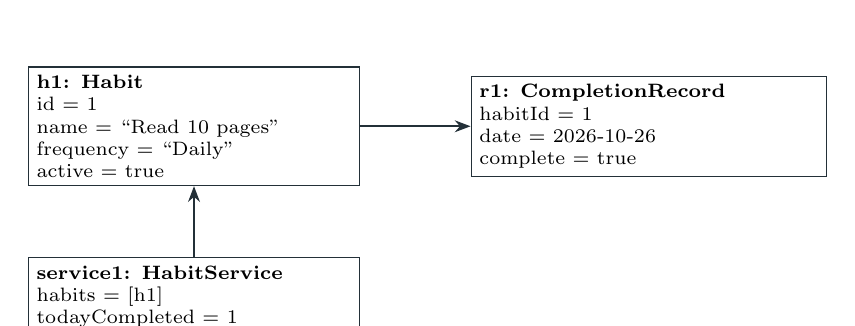
\begin{tikzpicture}[node distance=9mm and 14mm]
\node[uml,text width=40mm] (h1) {\textbf{h1: Habit}\\id = 1\\name = ``Read 10 pages''\\frequency = ``Daily''\\active = true};
\node[uml,right=of h1,text width=43mm] (r1) {\textbf{r1: CompletionRecord}\\habitId = 1\\date = 2026-10-26\\complete = true};
\node[uml,below=of h1,text width=40mm] (s1) {\textbf{service1: HabitService}\\habits = [h1]\\todayCompleted = 1};
\draw[arrow] (h1)--(r1);\draw[arrow] (s1)--(h1);
\end{tikzpicture}
\end{center}
This is an example runtime snapshot, not actual user data.

\section{Prototype Interface}
The first interface will be implemented in Java Swing. It will include a habit name field, frequency selector, add button, habit table, completion action, and a progress summary. The prototype uses at least five classes from the class diagram: \texttt{Main}, \texttt{Habit}, \texttt{CompletionRecord}, \texttt{HabitService}, \texttt{HabitRepository}, and \texttt{HabitTrackerFrame}. Source code is provided with this proposal.

\section{Implementation and Technology}
\begin{tabularx}{\linewidth}{lX}
\toprule
Component & Choice / purpose\\ \midrule
Language & Java 17+; object-oriented implementation.\\
GUI & Java Swing; desktop interface without external UI dependencies.\\
Persistence & Local serialized data file in the user's home directory (prototype); database may be considered in a later version.\\
Design & UI / service / repository separation.\\
Version control & Git and GitHub; commits grouped by feature or milestone.\\
Testing & Manual use-case tests plus unit tests for habit and summary logic where practical.\\
\bottomrule
\end{tabularx}

\section{Testing Plan and Acceptance Criteria}
\begin{tabularx}{\linewidth}{p{1.3cm}X X}
\toprule
Test ID & Test case & Expected result\\ \midrule
T-01 & Add a habit with a valid name & Habit appears in the list.\\
T-02 & Submit an empty name & Validation message appears; no habit is added.\\
T-03 & Mark a habit complete & Daily completion count and percentage update.\\
T-04 & Toggle the same habit again & Completion is undone without duplicate records.\\
T-05 & Close and reopen the app & Saved habits and logs remain available.\\
T-06 & Archive a habit & Habit is no longer shown as active; old records remain.\\
T-07 & Enter unusual characters in a name & App remains stable and displays the name safely.\\
\bottomrule
\end{tabularx}
Acceptance: all critical test cases pass, the app runs from a documented command, and the source and proposal are available in the GitHub repository.

\section{Risks and Mitigation}
\begin{tabularx}{\linewidth}{p{3.2cm}X}
\toprule
Risk & Mitigation\\ \midrule
Scope grows beyond the semester & Keep cloud, mobile, and social features out of version 1.\\
Persistence bugs & Test save/load repeatedly and keep repository logic isolated.\\
Limited development time & Deliver a working increment each week; prioritise core tracking.\\
UI and logic become coupled & Keep UI event handlers thin and use HabitService for rules.\\
\bottomrule
\end{tabularx}

\section{GitHub and Submission Checklist}
\begin{itemize}
\item \textbf{Repository:} \url{https://github.com/[username]/ovvasjatra} (replace placeholder with the actual repository URL).
\item Include this proposal PDF and its \LaTeX{} source.
\item Include Java source files, README with run instructions, and test checklist.
\item Add screenshots of the running prototype and meaningful Git commits.
\item Replace the cover-page placeholders before submission.
\end{itemize}

\section{Conclusion}
Ovvasjatra is a focused, achievable Java project that addresses habit consistency through habit management, daily completion records, and progress summaries. The iterative plan, requirements, six requested diagrams, schedule, testing plan, and Swing prototype provide a practical foundation for implementation and final demonstration.

\end{document}
